\section{Auswertung}
\label{sec:Auswertung}

\subsection{Magnetfeld von Spulen}
\subsubsection{Kurze Spule}
\label{sec:1}
In diesem Abschnitt wird die gemessene Magnetfeldstärke auf der radialsymmetrischen 
Achse von der kleinen und der großen Spule mit den theoretischen Werten für die 
erwartete Magnetfeldstärke verglichen.
\begin{table}[H]
    \centering
    \caption{Messwerte der kurzen Spule.}
    \label{tab:t1}
    %\sisetup{table-format=1.1, per-mode=reciprocal}
    \begin{tblr}{
        colspec = {S S},
        row{1} = {guard, mode=math},
      }
      \toprule
      \text{x} (\unit{\centi\meter}) & \text{Magnetfeldstärke} (\unit{\tesla}) \\
      \midrule
      0   &0.083\\
      1   &0.112\\
      2   &0.154\\
      3   &0.230\\
      4   &0.399\\
      5   &0.727\\
      6   &1.282\\
      7   &1.703\\
      8   &2.053\\
      9   &2.105\\
      10  &1.981\\
      11  &1.589\\
      12  &1.029\\
      13  &0.558\\
      14  &0.332\\
      15  &0.192\\
      16  &0.126\\
      \bottomrule
    \end{tblr}
\end{table}
\noindnet In \autoref{tab:t1} sind die aufgenommenen Messwerte der Magnetfeldstärke auf der Achse 
der kleinen Spule zu entnehmen. x ist der Abstand von einem Punkt 5 
\unit{\centi\meter} vor der Spule bis 5 \unit{\centi\meter} hinter der Spule.
Des weiteren sind die Messwerte in \autoref{fig:1} graphisch dargestellt.
\begin{figure}
    \caption{Magnetische Feldstärke auf der Achse der kurzen Spule}
    \label{fig:1}
    \centering
    \includegraphics{"build/plot1.pdf"}
\end{figure}
In Anbetracht der Tatsache, dass der Eintritt der Hall-Sonde in das Magnetfeld
5 \unit{\centi\meter} von $x = 0$ entfernt liegt und genau so nach dem Austritt
$5$ weitere Messwerte aufgenommen wurden, können die restlichen Messwerte, 
die in der Spule aufgenommen wurden, mitteln. Jenes dient dazu, das Magnetfeld 
im Inneren der Spule zu berechnen. Damit wird eine Feldstärke von 
\begin{equation*}
    B_{exp} = \qty{1.63(0.18)}{\milli\tesla}
\end{equation*}
erreicht. Die theoretische Magnetfeldstärke im Inneren der Spule kann mit
\autoref{eqn:4} bestimmt werden. Mit den Werten $I = 1 \unit{\ampere}$,
$n = 100$ und einer Länge von etwa 8 \unit{\centi\meter}
ergibt sich 
\begin{equation*}
    B_{theo} = \qty{1.57e-3}{\tesla} = \qty{1.57}{\milli\tesla}
\end{equation*}

%%%%%%%%%%%%%%%%%%%%%%%%%%%%%%%%%%%%%%%%%%%%%%%%%%%%%%%%%%%%%%%%%%%%%%%%%%%%%%%%%%%%%%%%%%%%%%%%%
\subsubsection{Lange Spule}
Bei der Ermittlung der Magnetfeldstärke in der langen Spule wird genauso
verfahren, wie schon in \autoref{sec:1}.
\begin{table}[H]
    \centering
    \caption{Messwerte der langen Spule.}
    \label{tab:t2}
    %\sisetup{table-format=1.1, per-mode=reciprocal}
    \begin{tblr}{
        colspec = {S S},
        row{1} = {guard, mode=math},
      }
      \toprule
      \text{x} (\unit{\centi\meter}) & \text{Magnetfeldstärke} (\unit{\tesla}) \\
      \midrule
      0   &0.019\\
      1   &0.041\\
      2   &0.072\\
      3   &0.136\\
      4   &0.253\\
      5   &0.503\\
      6   &0.971\\
      7   &1.544\\
      8   &1.978\\
      9   &2.192\\
      10  &2.279\\
      11  &2.333\\
      12  &2.360\\
      13  &2.379\\
      14  &2.382\\
      15  &2.379\\
      16  &2.368\\
      17  &2.340\\
      18  &2.301\\
      19  &2.231\\
      20  &2.286\\
      21  &2.184\\
      22  &1.965\\
      23  &1.552\\
      24  &0.977\\
      25  &0.519\\
      26  &0.297\\
      27  &0.190\\
      28  &0.133\\
      29  &0.101\\
      30  &0.081\\
      \bottomrule
    \end{tblr}
\end{table}

\begin{figure}
    \caption{Magnetische Feldstärke auf der Achse der langen Spule.}
    \label{fig:1}
    \centering
    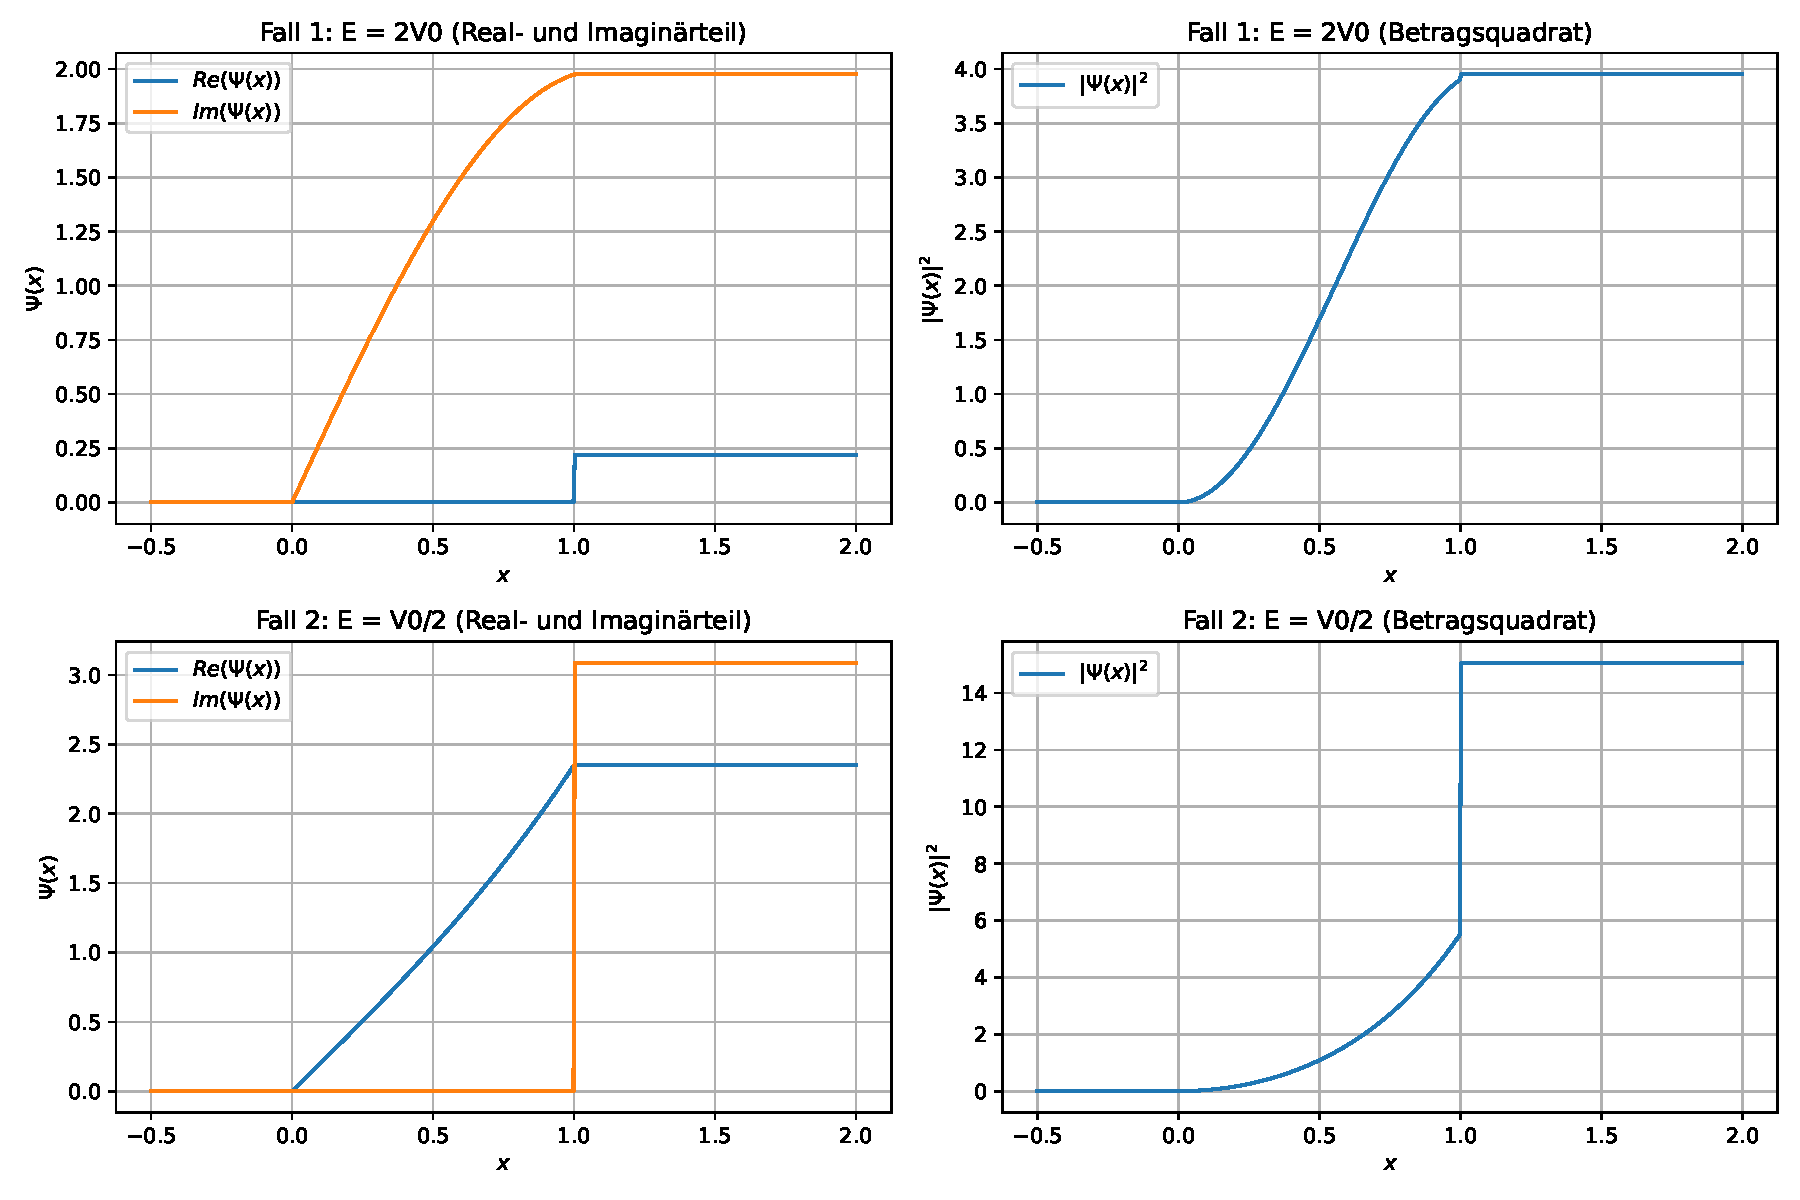
\includegraphics{"build/plot2.pdf"}
\end{figure}
\noindent Aus den Messwerten kann analog zu der kleinen  Spule das Magnetfeld
innerhalb der Spule gemittelt werden, um einen experimentellen Wert für die 
Magnetfeldstärke im inneren der Spule zu erhalten. Es ergibt sich
\begin{equation*}
    B_{exp,lang} = \qty{1.90(0.13)}{\milli\tesla}.
\end{equation*}
Der Theoretische Wert der Spule mit Länge $l = 19\unit{\centi\meter}$ wird
nach \autoref{eqn:4} bestimmt und beläuft sich auf
\begin{equation*}
    B_{exp,lang} = \qty{1.98e-3}{\tesla} = \qty{1.98}{\milli\tesla}.
\end{equation*}

%%%%%%%%%%%%%%%%%%%%%%%%%%%%%%%%%%%%%%%%%%%%%%%%%%%%%%%%%%%%%%%%%%%%%%%%%%%%%%%%%%%%%%%%%%%%%%%%%%%%%
\begin{table}[H]
    \centering
    \caption{Messwerte Hysteresekurve.}
    \label{tab:t3}
    %\sisetup{table-format=1.1, per-mode=reciprocal}
    \begin{tblr}{
        colspec = {S S },
        row{1} = {guard, mode=math},
      }
      \toprule
      I (\unit{\ampere}) & B(\unit{\milli\tesla}) \\
      \midrule
      0 &  1\\
    1  & 90\\
    2  & 260\\
    3  & 390\\
    4  & 479\\
    5  & 540\\
    4  & 516\\
    3  & 483\\
    2  & 430\\
    1  & 308\\
    0  & 122\\
    -1 & -80\\
    -2 & -258\\
    -3 & -395\\
    -4 & -482\\
    -5 & -540\\
    -4 & -515\\
    -3 & -483\\
    -2 & -429\\
    -1 & -305\\
    0  & -117\\
    1  & 79\\
    2  & 259\\
    3  & 392\\
    4  & 479\\
    5  & 340 \\
    \bottomrule
    \end{tblr}
\end{table}
\subsection{Hysteresekurve}
Über die aufgenommenen Messwerte der Magnetfeldstärke im Luftspalt der Ringspule
soll hier die Sättigungsmagnetisierung, Remanenz und Koerzitivkraft bestimmt
werden.
\begin{figure}[H]
    \caption{Hysteresekurve}
    \label{fig:3}
    \centering
    \includegraphics{"build/plot3.pdf"}
\end{figure}
Die Werte der Remananz kann man der Tabellle \autoref{}





%%%%%%%%%%%%%%%%%%%%%%%%%%%%%%%%%%%%%%%%%%%%%%%%%%%%%%%%%%%%%%%%%%%%%%%%%%%%%%%%%%%%%%%%%%%%%%%
Den Tabellen \autoref{} und \autoref{} sind die Werte für die Magnetfeldstärke auf der 
Symetrieachse eines Helmholzspulenpaares einmal für große und einmal für kleine 
Abstände der Spulen zu entnehmen. $x$ in $\unit{\milli\meter} $ ist dabei der Abstand 
vom linken ende der skala der Hall Sonde. Um die Darstellung und den Vergleich mit der 
Theoriekurve zu vereinfachen wurde die $x$-Skala so verschoben, dass der Nullpunkt jewails 
in der Mitte der beiden Spulen liegt.
\subsection{Helmholzspulenpaar}
\begin{figure}
    \caption{Magnetfeldstärke Spulenpaar $19\unit{\centi\meter}$ Abstand}
    \label{fig:4}
    \centering
    \includegraphics{"build/plot4.pdf"}
\end{figure}

\begin{figure}
    \caption{Magnetfeldstärke Spulenpaar $8\unit{\centi\meter}$ Abstand}
    \label{fig:5}
    \centering
    \includegraphics{"build/plot5.pdf"}
\end{figure}